\section{Colored Petri Net-based Analysis Model}
\label{sec:CPN_Modeling}

This section briefly describes how CPN can be used to build an extensible, scalable analysis model for component-based software applications. %In the context of the component model and the OS scheduler described in Section \ref{sec:Background}, this involves capturing (1) the nature of temporal partitioning, (2) properties of the component executor threads, (3) priority-based scheduling of the component executor threads, and finally, (4) using knowledge of the component's business logic code to model the scheduling of component operations. 
To edit, simulate and analyze this model, we use the CPN Tools 4 \cite{CPNTools} tool suite.  

\subsection{Model of Time}
\label{sec:model_of_time}

Appropriate choice for temporal resolution is a necessary first step in order to model and analyze threads running on a processor. The lowest-level OS scheduler enforces temporal partitioning and uses a priority-based scheme for threads active within a partition. The highest priority ready thread is always chosen first for execution. This thread keeps hold of the CPU as long as it is runnable and there are no other threads of same priority that need to run. If multiple threads have the same priority, Round-Robin (RR) scheduling  is enforced. Here, the scheduler allots a small quantum of time to one of the ready threads after which the thread is preempted by another ready thread of same priority. In order to observe and analyze this behavior, we have chosen the temporal resolution to be 1 ms (a fraction of 1 clock tick of the system timer). Since the temporal resolution is set as a global integer variable in the model, this value can be raised or lowered depending on the nature of the system being analyzed. 

\subsection{Modeling Temporal Partition Scheduling}
\label{sec:Modeling_Temporal_Partition_Scheduling}

Figure \ref{fig:cpn_tps} shows how the temporal partitioning is modeled using CPN. Each minor frame is modeled as a record color-set consisting of a partition number, a period, a duration and an offset. Aggregate of such minor frame tokens can fully describe a partition schedule. Complete partition schedules are maintained per computing node.

\vspace{-0.08in}
\begin{figure}[ht]
\centering
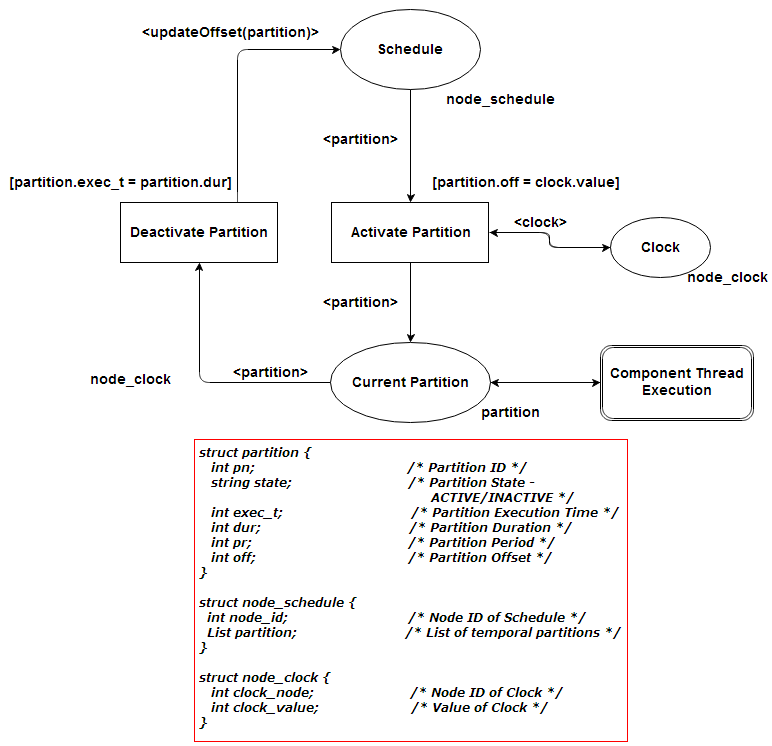
\includegraphics[width=0.40\textwidth]{cpn_tps}
\caption{CPN Model for Temporal Partition Scheduling}
\label{fig:cpn_tps}
\vspace{-0.2in}
\end{figure}
\vspace{0.05in}

Assuming that the partition scheduling shown in Figure \ref{fig:partition_scheduling} is imposed on the OS scheduler in node 1, the \emph{node\_schedule} token corresponding to this schedule is shown in Figure \ref{fig:cpn_tps_token}. This token populates the \emph{Schedule} place and decides the order of partition scheduling. When the node clock reaches the offset of one of these partitions, a valid binding is realized in order to fire the \emph{Activate Partition} which chooses the appropriate partition token and declares it as the \emph{Current Partition}. This active partition behaves as a constraint on the set of runnable component executor threads. \emph{Component Thread Execution} is a hierarchical transition that handles execution of component threads 1 ms at a time. At each millisecond, the \emph{exec\_t} field of the partition is updated. When this count reaches the duration of the partition, the offset of the partition is incremented by its period and the partition is made inactive. The above sequence of steps repeats for each partition.

\vspace{-0.08in}
\begin{figure}[ht]
\centering
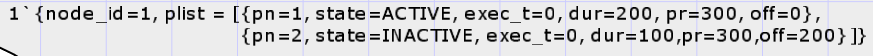
\includegraphics[width=0.5\textwidth]{cpn_tps_token}
\caption{CPN Token corresponding to Figure \ref{fig:partition_scheduling}}
\label{fig:cpn_tps_token}
\vspace{-0.18in}
\end{figure}
%\vspace{0.1in}
   
\subsection{Modeling Component Thread Behavior}
\label{sec:Modeling_Component_Thread_Lifecycle}

Figure \ref{fig:cpn_ctecycle} presents a simplified version of the CPN to model the thread execution cycle. The place \emph{Component\_Threads} holds \emph{node\_threads} tokens that keep track of all the ready threads in each computing node. Each thread is a record characterized by the node ID, thread ID, partition number, priority, start time of execution and state of currently executing operation. If multiple threads belonging to the same temporal partition are ready, the highest priority thread is chosen for execution. 

If the the highest priority thread is not already servicing an operation request, the highest priority operation from the \emph{Component Message Queue} is dequeued and scheduled for execution. The scheduled thread is placed in \emph{Currently Running Thread}. The guard on \emph{Schedule Thread} ensures that the highest priority ready thread belonging to the \emph{Current Partition} is always scheduled first. 

When a thread token is placed in \emph{Currently Running Thread}, the model checks to see if the thread execution has any effect on itself or on other threads. For instance: When the thread executes an operation that performs an RMI call, the effect of completion of the query is that the thread is moved to a blocked state and cannot run again till it receives a response from the server running on another thread. Such state changes are updated by the model using the \emph{Execute Thread} transition which also progresses time by 1 ms each time it fires. Keeping track of the node clock value, the thread is preempted at each clock tick. This loop repeats as long as there are no complete deadlocks in the system. 

\begin{figure*}
\centering
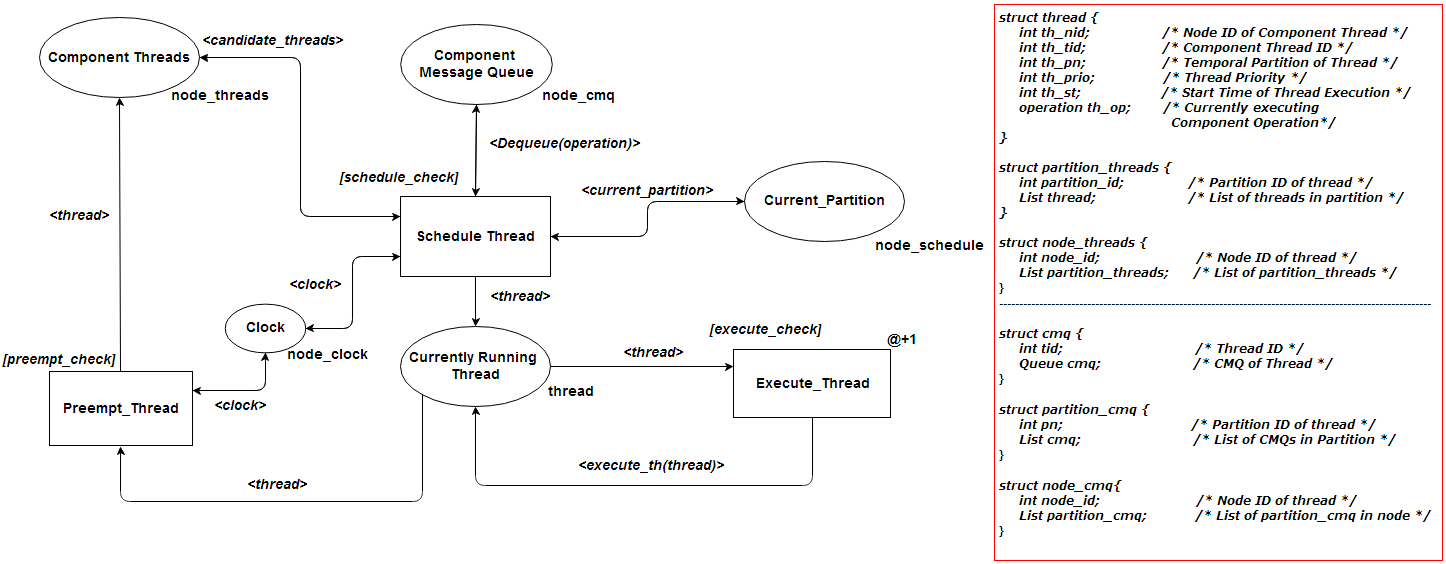
\includegraphics[width=\textwidth]{cpn_ctecycle}
\caption{Component Thread Execution Cycle}
\label{fig:cpn_ctecycle}
\vspace{-0.2in}
\end{figure*}

\subsubsection{Timer Operations}
\label{sec:Timer_Operations}

DREMS components are dormant by default. Once deployed, a component executor thread is not eligible to run until there is an operation added to the component's message queue. 

To start a sequence of component interactions, periodic or sporadic timers can be setup to trigger a component. When the component's timer expires, a timer-related operation is placed on the component message queue. When the component executor thread is picked by the OS scheduler, this operation is dequeued and the timer callback is executed. In CPN, timer operations are modeled as shown in Figure \ref{fig:cpn_timers}. 

\begin{figure}[ht]
\centering
\vspace{-0.1in}
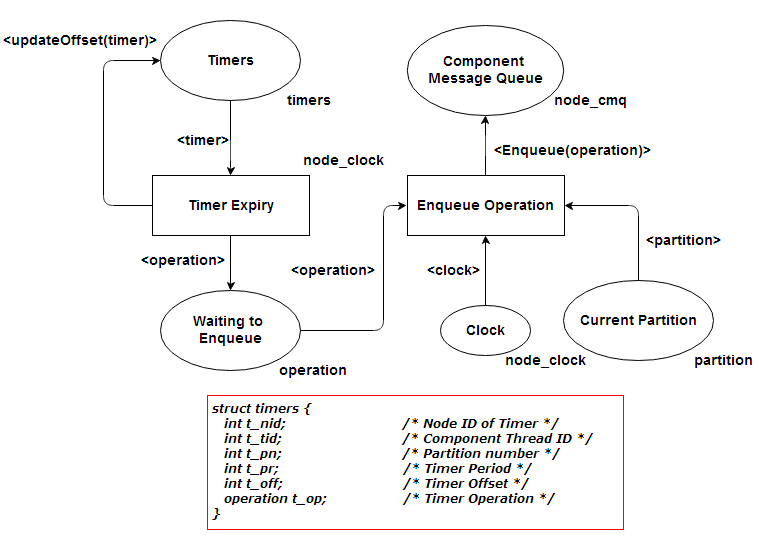
\includegraphics[width=0.5\textwidth]{cpn_timers}
\caption{Timer Operations}
\label{fig:cpn_timers}
\vspace{-0.17in}
\end{figure}

Every timer color-set token consists of a node ID, a thread ID, partition number, a period, an offset relative to the global node-specific clock, and an associated operation. The node ID, thread ID and partition number are necessary to correctly handle the enqueue action. All the component timers are expressed as separate tokens and initialized in the \emph{Timers} place. Notice that the enqueue operation does not happen until the appropriate partition is active. This is because the component-specific thread responsible for enqueueing incoming operations is also affected by temporal partitioning. 

\subsection{Modeling Component Operations}
\label{sec:Modeling_Component_Operations}

\vspace{-0.1in}
\begin{figure}[ht]
\centering
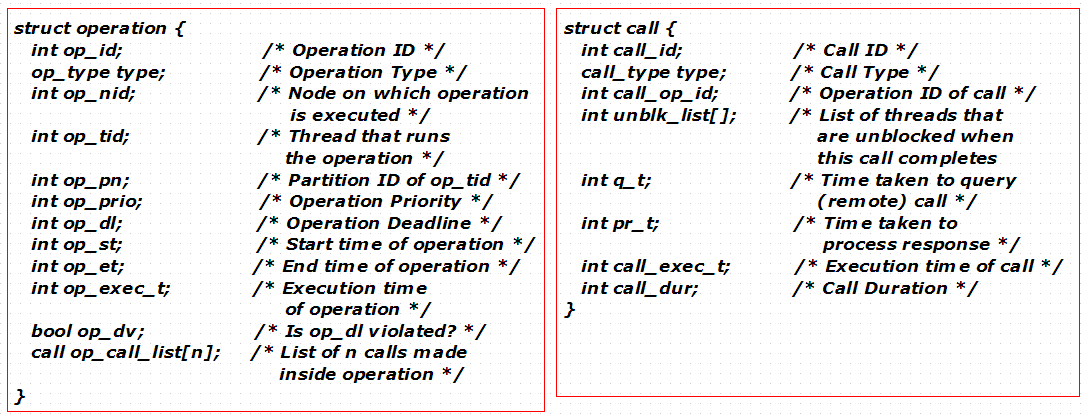
\includegraphics[width=0.5\textwidth]{cpn_operations}
\caption{Color-set for Component Operations}
\label{fig:cpn_operations}
\vspace{-0.2in}
\end{figure}
\vspace{0.1in}

As shown in Figure \ref{fig:cpn_operations}, every component operation is modeled as a record color-set in CPN. This record consists of the operation ID, operation type, node ID, thread ID, partition number, priority, deadline, temporal behavior and a list of function calls that represent the business logic of the execute function. New operations are inserted into the component message queue based on priority. The time stamp \emph{op\_st} is a snapshot of the node clock value when the operation is enqueued onto the message queue. The time stamp \emph{op\_et} is a snapshot of the node clock value when the operation is completed. Accounting for the wait-time in the message queue, the total execution time of the operation is compared against its deadline \emph{op\_dl}.

Once an operation is dequeued, the execution of the operation can be treated as a transition system that runs through a sequence of function calls dictating its behavior. Any of these underlying function calls can have a state-changing effect on the thread executing this operation. Consider a simple RMI application show in Figure \ref{fig:rmi_application}. The application has two components, a client and a server. The client component is associated with a timer that triggers a sequence of interactions between the two components. When the client timer expires, a timer operation is enqueued on the client's operation queue. When scheduled, the client executor thread executes this operation, which makes an RMI call to the server component. Once the query is made, the client thread is effectively blocked till a response is received. The server thread that produces this response may not be scheduled immediately due to the constraints of temporal partition scheduling. Once the RMI operation is completed on the server, the client thread is unblocked. 

\begin{figure}[ht]
\centering
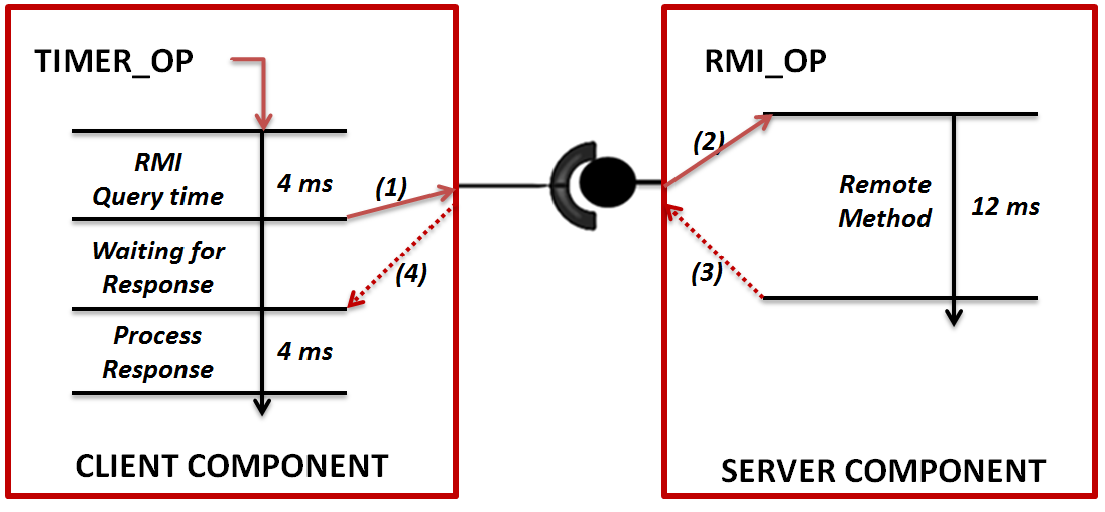
\includegraphics[width=0.4\textwidth]{rmi_application}
\caption{RMI Application}
\label{fig:rmi_application}
\vspace{-0.2in}
\end{figure}
\vspace{0.1in}

In the above example, the duration of time for which the client is blocked, is dependent on what happens inside the remote method on the server. This remote method could either simply take up CPU time, interact with the underlying framework or interact with other components in the application. To capture such interaction patterns, the \emph{call} color-set (Figure \ref{fig:cpn_operations}) is defined in CPN. Each call is identified by a \emph{call\_id} and a \emph{call\_type}. The field \emph{unblk\_list} is a list of threads that are unblocked when the call completes. This field is applicable to the RMI call completion on the server side which unblocks the client thread. Temporal behavior is captured using the last four fields: \emph{q\_t} is the worst-case estimate time taken for completion of a query; \emph{pr\_t} is the worst-case estimate time taken to process a response; \emph{call\_dur} is the effective duration of the call and \emph{call\_exec\_t} keeps track of how much of the call is complete. 

In the context of the earlier RMI example, two \emph{operation} tokens are required to describe the operations handled by the components: a client side timer operation and a server side RMI operation. A sample client timer operation is shown in Figure \ref{fig:cpn_rmi_app_timer_token}.

\vspace{-0.08in}
\begin{figure}[ht]
\centering
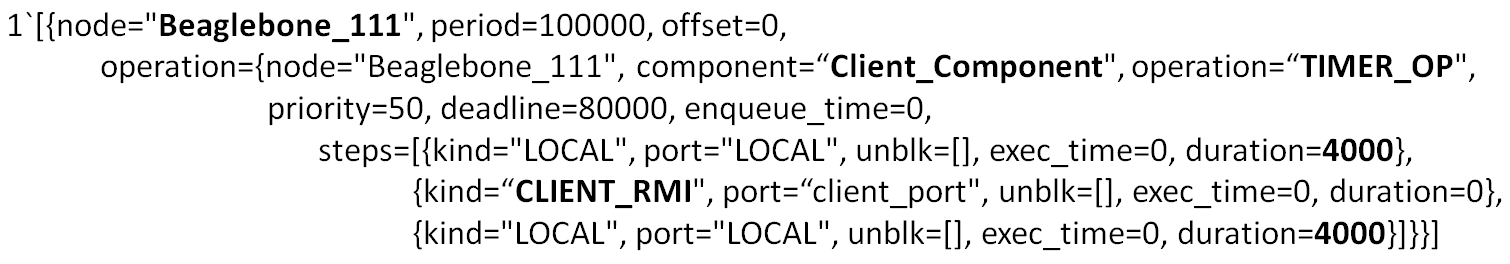
\includegraphics[width=0.5\textwidth]{cpn_rmi_app_timer_token}
\caption{RMI Application - Client Timer Operation}
\label{fig:cpn_rmi_app_timer_token}
\vspace{-0.16in}
\end{figure}


This timer operation runs on the client component (thread 1, partition 1) with a priority of 50, and a deadline of 80 ms. The business logic of this operation consists of a single RMI call that takes 4 ms to send out the query after which it blocks the executing client thread. After the client thread runs for time \emph{t = q\_t}, the client thread is moved to a blocked state and an RMI operation is induced on the server side. The client side thread remains blocked until the server thread completes executing the remote method. Once the server thread completes execution, it sends the response of the RMI back to the client. The model takes note of how long the client has been blocked by using the time stamp at which it receives a response. The client thread runs for an additional \emph{t = pr\_t} to process this response before it marks completion. The token for the server RMI operation is shown in Figure \ref{fig:cpn_rmi_app_server_token}.

%\vspace{0.1in}

This RMI operation is run on the server component (thread 2, partition 2) with a priority of 50 and a deadline of 80 ms. The deadline of this operation cannot be worse than the deadline of the client side operation that initiated the interaction. If this operation delays past 80 ms, a client side deadline violation is realized as the client thread is blocking for longer than expected. 

\vspace{-0.08in}
\begin{figure}[ht]
\centering
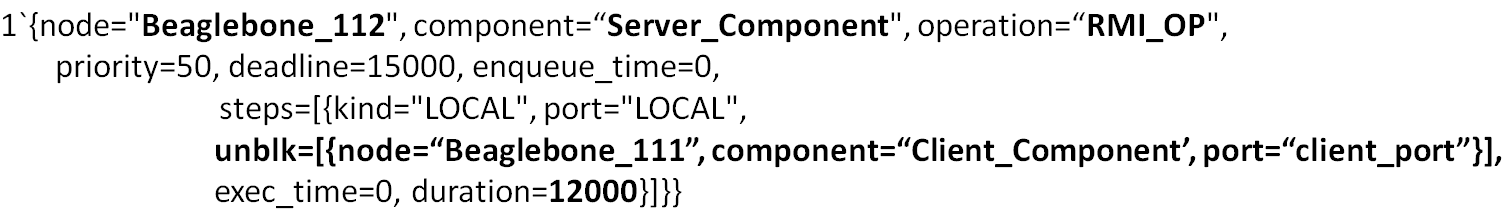
\includegraphics[width=0.5\textwidth]{cpn_rmi_app_server_token}
\caption{RMI Application - Server Operation}
\label{fig:cpn_rmi_app_server_token}
\vspace{-0.14in}
\end{figure}

\subsubsection{Induced Operations}
\label{sec:Operation_Induction}

To handle interactions between components, we take advantage of the developer's knowledge of the structure of the application, i.e, the component wiring. In the earlier example, we know that when the client executes an instance of a timer operation, a related RMI operation is enqueued on the server. In reality, this is handled by the underlying middleware. Since we do not model the details of this framework as of now, Figure \ref{fig:cpn_iop} shows how the CPN model induces operations on components based on the state of the currently running thread. 

Every \emph{induced\_operation} token contains a call ID and an operation. The transition \emph{Induce} observes the activity on the currently running thread. When initiating the model, if a particular call executed by a component thread would, on completion, request the services of another component, a token is placed on the \emph{Induce Operation} place. 

\vspace{-0.06in}
\begin{figure}[ht]
\centering
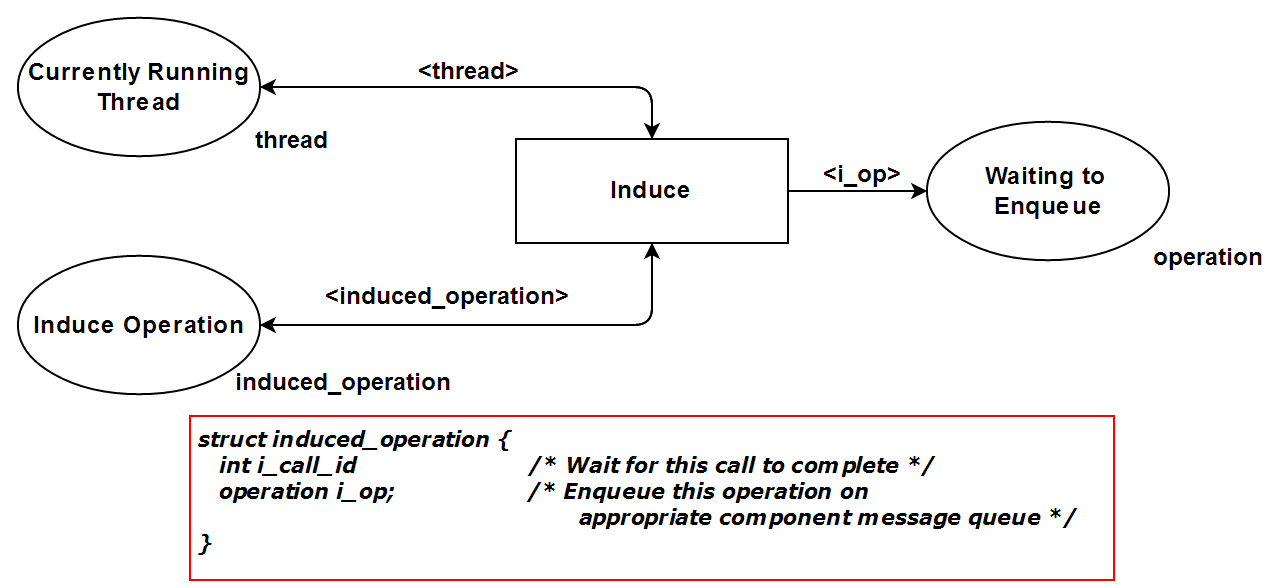
\includegraphics[width=0.5\textwidth]{cpn_iop}
\caption{Operation Induction}
\label{fig:cpn_iop}
\vspace{-0.14in}
\end{figure}
%\vspace{0.1in}

For the earlier RMI example, once the client thread pushes out an RMI query, an operation needs to be induced on the server queue. So an \emph{induced\_operation} token for this interaction is constructed. The model waits for the RMI call on the client side (call ID 1) to complete, at which point it places the operation \emph{i\_op} on the server message queue. This induction is represented in Figure \ref{fig:cpn_rmi_app_iop}. 

\vspace{-0.08in}
\begin{figure}[ht]
\centering
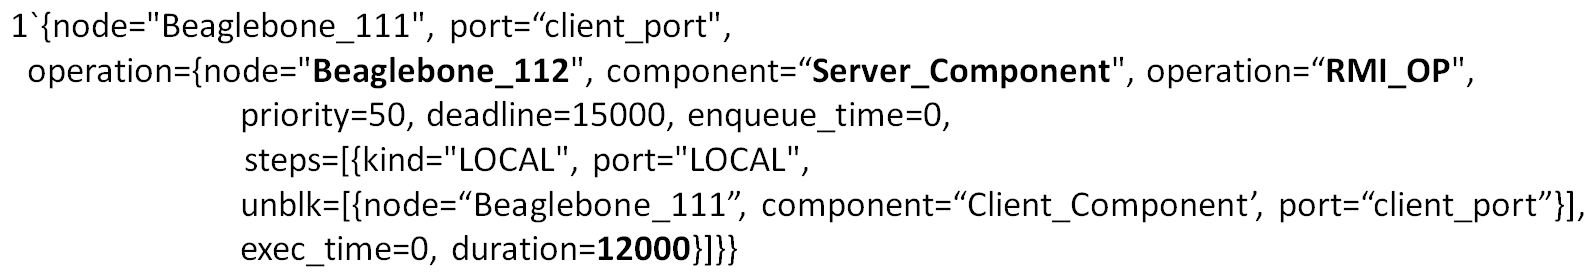
\includegraphics[width=0.5\textwidth]{cpn_rmi_app_iop}
\caption{Operation Induction Token}
\label{fig:cpn_rmi_app_iop}
\vspace{-0.16in}
\end{figure}

In this token, \emph{i\_call\_id = 1} represents the RMI call on the client. When the client thread is the currently running thread, it runs for as long as required to push out the RMI query. At this point, the \emph{Induce} transition becomes enabled and the RMI operation \emph{i\_op} is placed in \emph{Waiting for Enqueue}, eventually getting serviced. When initializing the model, a token is placed on \emph{Induce Operation} for every component interaction in the system, all of which are known ahead of time when the developer designs the application.